\documentclass[a4paper, 12pt]{report}
\usepackage{lmodern}
\pagestyle{plain}
%\usepackage{textcomp}
%\usepackage{tikz}
\usepackage[table]{xcolor}
\newcommand*\circled[1]{\textcircled{\footnotesize#1}\normalsize}
\usepackage[T1]{fontenc}
\usepackage{polski}
\usepackage[utf8]{inputenc}
\usepackage{graphicx}
\usepackage{wrapfig}
\newcommand\blankpage{\newpage \null \thispagestyle{empty} \addtocounter{page}{-1}}
%\usepackage[margin=4cm]{geometry}
\author{lek. Maciej Piwoda}
\title{Ostre Zapalenie Trzustki}
\begin{document}
\date{}
\maketitle
\blankpage
\tableofcontents
\thispagestyle{empty}
\addtocounter{page}{-1}
\blankpage
\chapter*{Wstęp}
\addcontentsline{toc}{chapter}{Wstęp}
{\sl,,Acute pancreatitis is the most terrible of all the calamities
that occur in connection with the abdominal viscera.''
\newline
\newline
,,Ostre zapalenie trzustki jest najgorszą katastrofą jaka może mieć
miejsce w jamie brzusznej''}
{\flushright{\hfill Sir Berkeley Moynihan\footnote{Brytyjski
      chirurg. W latach 1910-1927 kierował Katedrą Chirurgii Uniwersytetu w Leeds.}, 1925}}
\newline
\newline
\newline
\begin{indent}
Ostre zapalenie trzustki jest dość złożoną chorobą o bardzo
różnorodnym przebiegu klinicznym. Zapadalność w przeliczeniu na 100
tys. mieszkańców mieści się w szerokim zakresie: od ok 6 w Anglii do
80 w USA. Według niektórych badań\cite{7} występuje sezonowość zachorowań.
Szczyt zachorowań przypada w okresie wiosny i jesieni.
Mężczyźni chorują częściej niż kobiety (prawdopodobnie z powodu
częstszego nadużywania alkoholu, który jest jedną z głównych przyczyn
ostrego zapalenie trzustki).

U większości pacjentów przebieg choroby jest łagodny. U około 20-30\%
pacjentów rozwija się jednak ciężka postać choroby, wymagająca pobytu
w oddziale intensywnej terapii. Śmiertelność w tych przypadkach jest
wysoka i wynosi mniej więcej 30\%. Ogólna śmiertelność wśród
wszystkich chorych hospitalizowanych wynosi około 10\%.

Ostre zapalenie trzustki jako odrębna jednostka chorobowa zostało
opisane po raz pierwszy przez szwajcarskiego lekarza
Teofila Bonetusa w 1664 roku. Opie i Elliott w 1901 roku stworzyli teorię
,,wspólnego kanału'', według której głównym mechanizmem ostrego
zapalenia trzustki miało być mieszanie się soku trzustkowego z żółcią
w drogach żółciowych, a następnie jego zarzucanie do przewodu
trzustkowego. Zgodnie z teorią ,,toksemii enzymatycznej'' opracowanej
przez Bernarda w 1966 roku enzymy trzustkowe oraz częściowo produkty ich działania,
obecne w wysięku otrzewnowym są wchłaniane do krążenia i tą drogą
docierając do odległych narządów mogą je uszkadzać.
\end{indent}

\chapter{Budowa i topografia trzustki}

Trzustka opisana została po raz pierwszy w pierwszej połowie III
w.p.n.e przez greckiego lekarza i anatoma Herofilusa. Żyjącemu kilka 
wieków później Rufusowi z Efezu trzustka przypominała mięsień,
dlatego nadał jej nazwę \textsl{pancreas} od greckich słów:
$\pi\alpha\nu$ (cały) i $\kappa\rho\epsilon\alpha\varsigma$ (mięso), 
czyli dosłownie: cała z mięsa\cite{bochenek}.

Trzustka pełni podwójną funkcję. Jest gruczołem trawiennym i
jednocześnie gruczołem wydzielania wewnętrznego. Jest narządem, w którym
morfologicznie można wyróżnić szerszy koniec, zwany głową, leżący po
prawej stronie kręgosłupa, który łączy się z trzonem za pośrednictwem
zwężonego odcinka, zwanego szyją lub cieśnią trzustki. Najniższa część
głowy trzustki nazywana jest wyrostkiem haczykowatym. Głowa leży na
wysokości I i II kręgu lędźwiowego i jest otoczona pętlą dwunastnicy. 
Trzon trzustki na górnym brzegu ma zgrubienie, zwane guzem sieciowym. Lewy koniec,
wznoszący się ku górze i sięgający wnęki śledziony to ogon trzustki.
Zarówno głowa, jak i ogon są spłaszczone w płaszczyźnie strzałkowej,
natomiast trzon jest trójgraniasty i posiada trzy powierzchnie:
przednią, tylną i dolną oraz trzy brzegi: przedni, górny i dolny.
Długość trzustki mieści się w zakresie 12 do 20 cm, masa to około 80
gramów. Jest narządem o miękkiej konsystencji, koloru szaroróżowego.

Głowa i trzon trzustki leżą pozaotrzewnowo, natomiast ogon
wewnątrzotrzewnowo, między blaszkami więzadła
przeponowo-śledzionowego
Tylna powierzchnia głowy trzustki przylega do prawej żyły i tętnicy
nerkowej, żyły czczej dolnej i do żyły wrotnej. Za głową lub w jej
miąższu przebiega przewód żółciowy wspólny. Naczynia krezkowe górne
biegną za szyją trzustki. Tylna powierzchnia trzonu z kolei przylega
do aorty, żyły krezkowej dolnej, żyły śledzionowej, naczyń nerkowych
lewych, lewego nadnercza i lewej nerki. Za ogonem trzustki znajduje
się natomiast górny biegun nerki lub śledziona. Do powierzchni
przedniej głowy przylega poprzecznica lub też korzeń jej krezki. Trzon
od przodu pokryty jest otrzewną, tworząc w ten sposób tylną ścianę
torby sieciowej, do której w tym miejscu przylega
żołądek. Powierzchnia dolna trzonu również pokryta jest otrzewną i za
jej pośrednictwem styka się z jelitem czczym. Nad brzegiem górnym
trzonu leży pień trzewny, od którego odchodzi tętnica śledzionowa
przebiegająca wzdłuż górnego brzegu trzustki, która następnie
wraz z żyłą śledzionową przechodzi na powierzchnię przednią ogona.
Trzustka jest narządem o budowie zrazikowej. Z każdego zrazika
odchodzi krótki przewodzik, uchodzący do przewodu
trzustkowego. Przewód ten ma swój początek w ogonie trzustki. Łączy
się on z przewodem żółciowym wspólnym i razem z nim uchodzi do
dwunastnicy na brodawce większej (Vatera). Z górnej części głowy trzustki
powstaje przewód trzustkowy dodatkowy, który czasami uchodzi
samodzielnie do dwunastnicy na brodawce mniejszej (Santoriniego), leżącej bardziej
dogłowowo w stosunku do brodawki większej.  Trzustka w krew
zaopatrywana jest przede wszystkim przez górną i dolną tętnicę trzustkowo-dwunastniczą
(głowa) i odgałęzienia tętnicy śledzionowej (trzon). Żyły trzustki,
odpowiadające tętnicom uchodzą do żyły wrotnej. Włókna autonomiczne
układu sympatycznego unerwiające trzustkę pochodzą ze splotu trzewnego lub od splotów
naczyniowych tętnic zaopatrujących trzustkę, natomiast unerwienie
parasympatyczne pochodzi od nerwu błędnego.

\begin{figure}[h!]
\centering
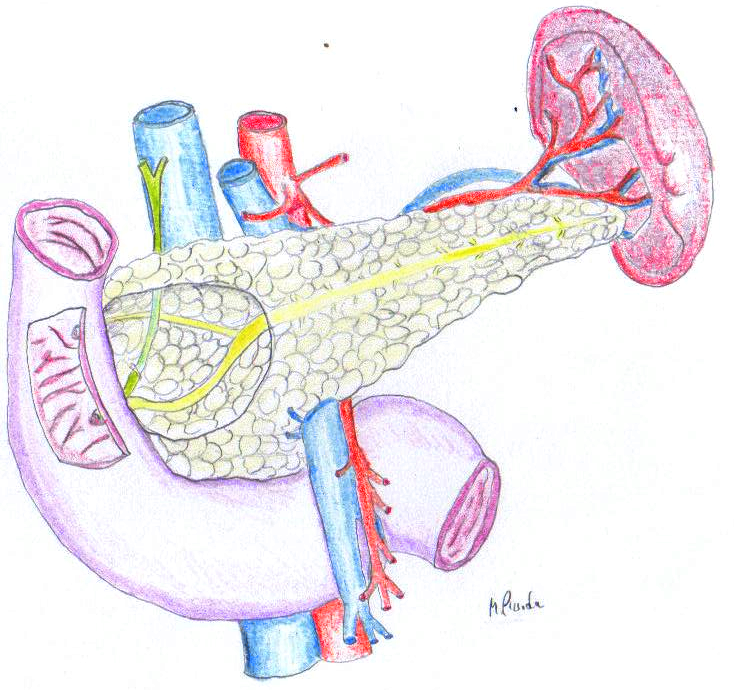
\includegraphics[scale=0.28]{pancreas}
\caption{Topografia trzustki}
\end{figure}

Trzustka jak wspomniano wcześniej ma budowę zrazikową. Około 85\%
masy tego narządu stanowią pęcherzyki wydzielnicze. Każdy z
pęcherzyków składa się z 20 do 50 nabłonkowych komórek pęcherzykowych,
które mają dość charakterystyczny kształt piramidy, u podstawy której
położone jest jądro, a u szczytu znajdują się ziarnistości zymogenowe,
których zawartość jest wydzielana do światła pęcherzyka. Wewnątrz
pęcherzyka znajdują się również mniejsze, płaskie komórki, które
tworzą wyściółkę na powierzchni komórek pęcherzykowych, a następnie
przechodzą w komórki kanalików wstawkowych i później przewodów
wyprowadzających sok trzustkowy do dwunastnicy. Komórki te wydzielają
wodę i elektrolity, głównie wodorowęglany. Z pęcherzyków odchodzą
przewody wyprowadzające, które się ze sobą łączą i ostatecznie uchodzą
do głównego przewodu trzustkowego.

\begin{figure}[h!]
\centering
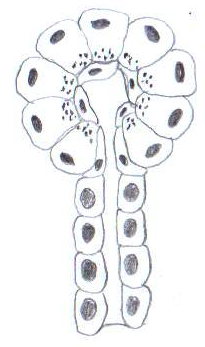
\includegraphics[scale=0.3]{zrazik}
\caption{Budowa zrazika}
\end{figure}

W trzustce znajdują się także tzw. wyspy trzustkowe (Langerhansa),
czyli skupiska komórek dokrewnych. Stanowią one zaledwie 2\% masy
miąższu trzustki i choć rozsiane są po całym narządzie, najwięcej
ich można znaleźć w obrębie ogona. Są one odpowiedzialne za
wydzielanie glukagonu (komórki A), insuliny (komórki B), somatostatyny
(komórki D) i polipeptydu trzustkowego (komórki F). Tętniczki
doprowadzające krew do wysp Langerhansa rozdzielają się na włośniczki
zatokowate, które otaczają komórki wysp, następnie pod postacią
mniejszych naczyń włosowatych zaopatrują pęcherzyki wydzielnicze. 
Stanowi to rodzaj krążenia wrotnego, dzięki któremu krew bogata w
hormony trzustkowe dociera do tkanki
zewnątrzwydzielniczej.\cite{szczeklik}\cite{traczyk}

\chapter{Fizjologia trzustki}
Trzustka jest narządem pełniącym w organizmie dwie zasadnicze
funkcje. Są to:
\begin{itemize}
\item[-] funkcja zewnątrzwydzielnicza, polegająca na produkcji soku
  trzustkowego, niezbędnego do właściwego trawienia pokarmów
\item[-] funkcja wewnątrzwydzielnicza, za którą odpowiadają wyspy
  Langerhansa
\end{itemize}

[tu schemat trzustka i co wydziela]

\section{Czynność zewnątrzwydzielnicza}
\subsection{Sok trzustkowy}
Sok trzustkowy wydzielany przez trzustkę do dwunastnicy jest płynem
izoosmotycznym i zasadowym (pH 8,0-8,5). W jego skład wchodzą enzymy
trawiące białka, tłuszcz, węglowodany i kwasy nukleinowe. Oprócz tego
zawiera on elektrolity i śluz. Jego dzienna produkcja wynosi od 1 do 4
litrów, w zależności od przyjmowanych pokarmów. Główne aniony soku
trzustkowego to jony: wodorowęglanowy (HCO$_3^-$) i chlorkowy
(Cl$^-$). Dzięki zasadowemu odczynowi neutralizuje on sok żołądkowy, 
co sprawia, że pH w dwunastnicy jest optymalne do działania enzymów
trzustkowych. Jony HCO$_3^-$ produkowane są przez anhydrazę węglanową
w komórkach śródpęcherzykowych i komórkach kanalików wyprowadzających.
Komórki pęcherzykowe natomiast syntetyzują i wydzielają enzymy
trawienne. W ciągu doby produkują ok 40g białka, które jest strawione
i następnie wchłonięte w jelitach\cite{szczeklik}.

Enzymy trzustkowe to w ok. 80\% enzymy proteolityczne: trypsyna,
chymotrypsyna, karboksypeptydazy A i B oraz elastaza. Enzymy te
wydzielane są w postaci nieaktywnych proenzymów: trypsynogenu, chymotrypsynogenu,
prokarbopeptydaz i proelastazy. Pod wpływem enterokinazy, wydzielanej
przez komórki nabłonka dwunastnicy proenzymy przekształcane są do
aktywnych postaci. Trypsyna również aktywuje inne zymogeny, włącznie z
trypsynogenem. Trypsyna i chymotrypsyna są endopeptydazami i
trawią białko do oligopeptydów, które są następnie rozkładane do
pojedynczych aminokwasów przez egzopeptydazy (karboksypeptydazy i
aminopeptydazy) oraz dipeptydazy jelitowe. Składnikiem soku
trzustkowego jest także inhibitor trypsyny, zwany SPINK1
(\textsl{serine protease inhibitor Kazal type I}).

[schemat z aktywacją proteaz]

Enzymy lipolityczne to: lipaza, fosfolipaza i esterazy. Lipaza
wydzielana jest w postaci czynnej i rozkłada ona triacyloglicerole do
kwasu tłuszczowego, monoacylogliceroli i glicerolu. Działa ona na
pograniczu fazy wodno-tłuszczowej, dlatego do swojego działania wymaga
obecności soli żółciowych, które działając jako detergent,
przekształcają krople tłuszczu w emulsję. Do właściwego działania
lipazy niezbędna jest także kolipaza - oligopeptyd, będący również
składnikiem soku trzustkowego, który łącząc się z trzustką zwiększa
jej aktywność lipolityczną, chroni ją przed proteolizą, obniża
optymalne dla lipazy pH z 8,5 do 6,5. Fosfolipaza jest natomiast
wydzielana w postaci nieczynnego prekursora (profosfolipazy), który
ulega aktywacji przez trypsynę. Rolą tego enzymu jest rozkład
fosfolipidów do kwasów tłuszczowych. Esterazy rozszczepiają estry karboksylowe, takie jak
estry cholesterolu i witamin rozpuszczalnych w tłuszczach.

Enzymem glikolitycznym jest $\alpha$-amylaza, wydzielana w postaci
czynnej. Zadaniem jej jest hydroliza wewnętrznych wiązań
$\alpha$-1,4-glikozydowych skrobi, rozkładając ją do maltozy,
maltotriozy oraz $\alpha$-dekstryn. Dalsza hydroliza do cukrów
prostych ma miejsce w obrębie rąbka szczoteczkowego enterocytów przy
udziale tam obecnych enzymów.

Pośród pozostałych enzymów soku trzustkowego najważniejsze są enzymy
nukleolityczne, czyli rybonukleaza i deoksyrybonukleaza, które
hydrolizując wiązania fosfodiestrowe kwasów nukleinowych, rozkładają
je na mono- i oligonukleotydy.

\subsection{Regulacja wydzielania trzustkowego}
Wydzielanie trzustkowe rozpoczyna się w chwili spożywania
pokarmu. Odpowiedź indukowana posiłkiem składa się z trzech faz:
głowowej, żołądkowej i jelitowej. Do struktur neuronalnych
sterujących funkcją zewnątrzwydzielniczą trzustki należą: mózg, nerw
błędny (jądro grzbietowe), układ współczulny, nerwy jelitowe
zaopatrujące trzustkę ze splotów śródściennych żołądka i dwunastnicy.
Hormony wydzielane przez komórki endokrynne wysp trzustkowych i jelit
odgrywają również ważną funkcję w regulacji czynności trzustki.

Obecność tłuszczów i białka w jelicie jest głównym bodźcem dla
wydzielania trzustkowego. Węglowodany indukują słabą odpowiedź,
natomiast alkohol może trzustkę stymulować albo hamować.
Cholecystokinina i sekretyna są hormonami odpowiedzialnymi za
pobudzanie wydzielania soku trzustkowego. Sekretyna jest wydzielana 
przez komórki S, znajdujące się w górnym odcinku jelita cienkiego, 
przy pH < 4,5. Pobudza ona komórki przewodów trzustkowych i
śródpęcherzykowe do wytwarzania dużych ilości płynu bogatego w wodoroweglany. 
Cholecystokinina jest natomiast uwalniana z komórek błony śluzowej
dwunastnicy w odpowiedzi na pojawienie się w dwunastnicy białek i
tłuszczów. Pobudza ona uwalnianie enzymów trzustkowych z komórek
pęcherzykowych. Nasila także działanie sekretyny.Cholecystokinina i
sekretyna działają na trzustkę pośrednio poprzez wiązanie się z
receptorami na włóknach aferentnych nerwu błędnego. Odruchy z nerwu
błędnego pełnią ważną rolę w kontroli czynności zewnątrzwydzielniczej
trzustki (szczególnie w fazie głowowej). Liczne odruchy
jelitowo-trzustkowe odpowiedzialne są za rozpoczęcie wydzielania
trzustkowego, w odpowiedzi na obecność pokarmu w jelicie cienkim.

Niezbyt wiele wiadomo na temat hamowania wydzielania soku
trzustkowego. Wydaje się, że istotny wpływ może mieć wysoki poziom
glukagonu w okresie po posiłku. To samo dotyczy somatostatyny i
wazoaktywnego peptydu jelitowego. Przypuszczalnie obecność enzymów
trzustkowych w świetle jelita zmniejsza wydzielanie trzustkowe poprzez
hamowanie uwalniania cholecystokininy.

Wydzielanie zymogenów z komórek pęcherzykowych odbywa się na dwa
sposoby. Większość z nich uwalnia jest przez błonę szczytową w wyniku
stymulacji neurohormonalnej. Około 15\% jednak uwalniane jest w sposób
konstytutywny, nie tylko przez błonę szczytową, ale także przez część
boczno-podstawną błony komórkowej. Tłumaczyć to może fizjologiczną
stałą obecność enzymów trzustkowych we krwi.

\section{Czynność wewnątrzwydzielnicza}

Komórki wysp Langerhansa wydzielają hormony regulujące metabolizm
węglowodanów, tłuszczy i białek. Hormony te to: insulina, glukagon,
somatostatyna, polipeptyd trzustkowy.

Insulina, wytwarzana przez komórki B wysp trzustkowych jest
polipeptydem, składającym się z dwóch łańcuchów aminokwasowych: A i B, 
połączonych mostkami dwusiarczkowymi. Insulina jest hormonem
anabolicznym. Działa przede wszystkim na mięśnie, wątrobę i tkankę tłuszczową.
Powoduje nasilenie wychwytu glukozy w tkance tłuszczowej i mięśniach,
syntezy glikogenu w wątrobie i miocytach, wychwytu aminokwasów przez
mięśnie i wzrost syntezy białek, przy jednoczesnym hamowaniu
katabolizmu białkowego. Nasila ona także syntezę kwasów tłuszczowych w
adipocytach i hepatocytach, oraz powoduje wzrost aktywności lipazy
lipoproteinowej w tkance tłuszczowej. Insulina odpowiedzialna jest
także za nasilenie wychwytu jonów potasu i fosforanów oraz hamowanie ketogenezy.

\begin{figure}[h]
\centering
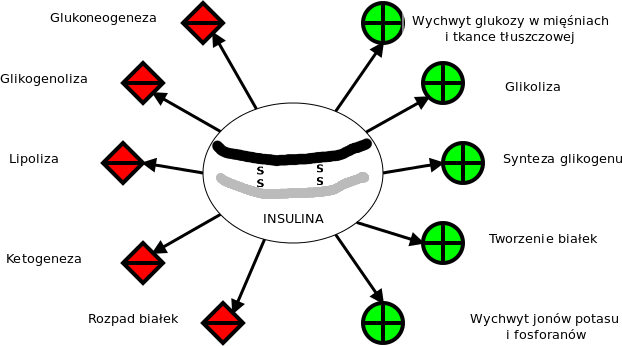
\includegraphics[scale=0.5]{Insulina_diag2}
\caption{Działanie insuliny}
\end{figure}

Glukagon jest polipeptydem produkowanym przez komórki A wysp
Langerhansa. Glukagon ma działanie antagonistyczne w stosunku do
insuliny. Jego podstawowym działaniem jest zwiększanie stężenia
glukozy we krwi. Stymuluje on glikogenolizę w wątrobie,
glukoneogenezę, lipolizę i ketogenezę.

Somatostatyna\footnote{ Somatostatyna jest wytwarzana także
w podwzgórzu jako czynnik hamujący hormon wzrostu (GH-IH).}jest
polipeptydem wydzielanym
przez komórki D. Istnieją w dwóch formach: SS14 i SS28, z których ta druga
jest bardziej aktywna. Somatostatyna hamuje wydzielanie insuliny,
glukagonu i polipeptydu trzustkowego. Wpływa także na perystaltykę,
powodując spowolnienie ruchów perystaltycznych w przewodzie
pokarmowym. Hamuje również wydzielanie soku żołądkowego, trzustkowego i
żółci.

Polipeptyd trzustkowy wytwarzany jest w komórkach F wysp trzustkowych. Jego
rola nie jest jeszcze dostatecznie poznana. Wiadomo, że obniża
stężenie glukozy i aminokwasów we krwi po posiłku. Ponadto zmniejsza
wydzielanie trzustkowe, hamuje kurczliwość pęcherzyka żółciowego,
pobudza wydzielanie żołądkowe i opóźnia opróżnianie żołądka.

\chapter{Ostre zapalenie trzustki - definicja i terminologia}

Ostre zapalenie trzustki jest to ostry stan zapalny będący wynikiem
aktywacji trzustkowych enzymów trawiennych w miąższu gruczołu,
sąsiadujących tkankach i niekiedy również w odległych narządach.
Zmianom lokalnym może towarzyszyć uogólniony odczyn zapalny (SIRS\footnote{definicja}) i
niewydolność wielonarządowa (MOF\footnote{kolejna definicja}). 

Sama choroba jak i jej powikłania mogą przebiegać w bardzo różnorodny
sposób, dlatego niezwykle trudne jest ustalenie jednolitej
terminologii. Najczęściej używana jest klasyfikacja z Atlanty, która
po raz pierwszy ukazała się w 1992 roku. W 2012 roku została ona
zrewidowana. 

Wyróżnia się obecne dwie fazy zapalenia trzustki: wczesną
i późną. Faza wczesna związana jest z SIRS i trwa około tygodnia, choć czasem może ulec
przedłużeniu do dwóch tygodni. Faza późna trwa od kilku tygodni do
nawet kilku miesięcy i cechuje się objawami ogólnymi trwającego
zapalenia, ogólnoustrojowymi i miejscowymi powikłaniami oraz
przetrwałą niewydolnością narządową. 

Definiuje się trzy stopnie ciężkości ostrego zapalenia
trzustki (tabela 1),  w zależności od chorobowości i śmiertelności. Jak
najszybsze określenie ciężkości choroby jest istotne ze wzgledu na
konieczność identyfikacji pacjentów, którzy będą wymagać agresywnego
leczenia. Dopiero po upływie 48 godz. jest możliwe odróżnienie
ciężkiego od średniego zapalenia trzustki, dlatego wszystkich
pacjentów z SIRS należy leczyć jakby mieli ciężką postać OZT.
\begin{table}[htbp]
\begin{center}
\begin{footnotesize}
\begin{tabular}{|p{4cm}|p{9cm}|}
\hline
\multicolumn{2}{|c|}{\cellcolor[gray]{0.9} \textbf{Tabela 1. Stopnie ciężkości ostrego zapalenia trzustki}}\\
\hline \hline
stopień łagodny & bez niewydolności narządowej i powikłań\\ \hline
stopień umiarkowany & przejściowa niewydolność narządowa (<48
                           godz.) i/lub powikłania miejscowe bądź
                           ogólnoustrojowe\\ \hline
stopień ciężki & przetrwała niewydolność narządowa dotycząca
                       co najmniej jednego układu (>48 godz.)\\ \hline
\multicolumn{2}{|l|}{\footnotesize{na podstawie: Banks i wsp.\cite{banks}}}\\
\hline
\end{tabular}
\end{footnotesize}
\end{center}
\end{table}

Ostre zapalenie trzustki można podzielić na dwa typy: śródmiąższowe
obrzękowe zapalenie trzustki i martwicze zapalenie trzustki. 

U przeważającej części chorych (80-90\%) występuje postać łagodniejsza,
czyli śródmiąższowe zapalenie trzustki. W badaniach obrazowych
widoczne jest zazwyczaj rozlane powiększenie trzustki, wynikające z
obrzęku zapalnego. Oprócz tego można również uwidocznić płyn w okolicy
okołotrzustkowej oraz zatarcie struktury i granic miąższu
trzustki. Nie występuje natomiast martwica. Ta postać zapalenia trwa
około tygodnia.

Martwicze zapalenie trzustki jest bardziej agresywną postacią
choroby. Cechuje się obecnością (jak sama nazwa wskazuje) martwicy
miąższu trzustki lub okolicznych tkanek. Rozpoznanie tej postaci
OZT za pomocą li tylko badań obrazowych może być niezwykle trudne
w pierwszym tygodniu choroby. W późniejszym okresie w obrazie TK
widoczne są w obrębie trzustki i/lub okolicznych tkanek niejednorodne
zbiorniki zawierające składniki lite i płynne. Martwicze zapalenie trzustki można
dodatkowo podzielić na jałowe i zakażone. W zakażonym, oprócz
utrzymujących się objawów i badań laboratoryjnych wskazujących na
infekcję, w obrazie TK można zobaczyć gaz poza światłem jelita - w
obrębie trzustki i/lub sąsiadujących tkanek. 

\chapter{Etiologia i patogeneza}

W krajach rozwiniętych za 75-80\% przypadków ostrego zapalenia
trzustki odpowiadają alkohol i kamica przewodów żółciowych. Wśród
innych, znacznie rzadszych przyczyn należy wymienić: leki
(kortykosteroidy, tiazydy, azatiopryna), jatrogenne (ERCP),
hiperlipidemia, hiperkalcemia, wady wrodzone (trzustka dwudzielna),
choroby dziedziczne (mukowiscydoza, rodzinne ozt), toksyczne (jad
skorpiona), pourazowe, niedokrwienne, dysfunkcja zwieracza Oddiego,
infekcyjne (świnka, HIV, cytomegalia, Coxackie, salmonelloza,
gruźlica, bruceloza, leptospiroza, glistnica), autoimmunologiczne
(toczeń rumieniowaty układowy, zespół Sjögrena). W około 10\% przypadków
ostrego zapalenia trzustki przyczyna jest nieznana. 

Ważny jest również wpływ czynników genetycznych, co udowodniono w
licznych badaniach w ostatnich latach.
Polimorfizm genowy wcześniej wspomnianego inhibitora trypsyny (SPINK1)
jest związany z większym ryzykiem wystąpienia tej choroby.\cite{38}
Podobnie jak i mutacja w genie białka
CTFR\footnote{\textsl{ang. cystic fibrosis transmembrane conductance 
regulator (CFTR)} - białko budujące kanał chlorkowy, jego
  nieprawidłowa forma jest przyczyną mukowiscydozy}.\cite{39}
Wykazano również związek między polimorfizmem genowym
czynnika-$\alpha$ martwicy nowotworu (\textsl{tumor necrosis factor -
TNF-$\alpha$}) i Hsp70 (\textsl{heat shock protein 70}) a większą
zachorowalność na ostre zapalenie trzustki.\cite{40}

Jak wspomniano wyżej najczęstszymi przyczynami ostrego zapalenia
trzustki są alkohol i kamica przewodów żółciowych. Dokładna patogeneza
wciąż nie jest do końca jasna. Wiadomo, że alkohol zwiększa
przepuszczalność nabłonka przewodu trzustkowego, dzięki czemu jest on
przepuszczalny dla większych cząstek. Tym sposobem enzymy trzustkowe
przechodzą do tkanki śródmiąższowej otaczającej przewód i tam wywołują
uszkodzenia. Wzrost ciśnienia w przewodzie trzustkowym może być spowodowany
wytrącaniem się białek, za co również odpowiada alkohol lub też przez
okluzję wywołaną kamicą przewodową, w której ponadto dochodzi do
zarzucania żółci, niszczącej nabłonek przewodu.

Niezależnie od przyczyny dominującą rolę w rozwoju choroby pełni
trypsyna, której działanie w postaci przedwczesnej aktywacji enzymów
trzustkowych prowadzi do samotrawienia trzustki i tkanek
okołotrzustkowych. Za aktywację trypsynogenu wewnątrz komórek
pęcherzykowych odpowiadać może min. zwiększone stężenie jonów wapnia,
czy lizosomalna katepsyna B.\cite{21} 

Trzustkowe komórki pęcherzykowe
giną w wyniku nekrozy lub apoptozy. W wyniku nekrozy dochodzi lizy
komórek i uwalniania zawartości wewnątrzkomórkowej, co prowadzi do
wystąpienia reakcji zapalnej. Dochodzi do aktywacji (również wskutek
bezpośredniego działania trypsyny) licznych
mediatorów zapalnych, układu kinin, dopełniacza, krzepnięcia i
fibrynolizy. Neutrofile, makrofagi, limfocyty naciekają podścielisko
łącznotkankowe trzustki i po aktywacji stanowią kolejne źródło
mediatorów zapalnych. Może to prowadzić do przejścia zlokalizowanego
zapalenia w zespół ogólnoustrojowej reakcji zapalnej (\textsl{systemic inflammatory response
  - SIRS}), z obecnością tych samych zmian w mikrokrążeniu,
przepuszczalności śródbłonka i działaniu mediatorów zapalnych jak w
sepsie. 

W przeciwieństwie do nekrozy, apoptoza nie wywołuje
reakcji zapalnej. Komórki są degradowane do pęcherzyków otoczonych
błoną komórkową, które są pochłaniane przez makrofagi. Fagocytoza
komórek, które uległy apoptozie nie tylko zapobiega miejscowemu
zapaleniu, ale powoduje też zwiększoną produkcję interleukiny 10
(\textsl{IL-10}), będącą czynnikiem antyzapalnym. W ostrym zapaleniu
trzustki o ciężkim przebiegu poziom IL-10 jest znacznie
zmniejszony,\cite{27} natomiast zwiększoną ilość kaspaz, czyli białek
odpowiadających za apoptozę obserwuje się w łagodniejszych postaciach
tej choroby.\cite{26}

Aktywowane enzymy trzustkowe uszkadzają nie tylko komórki
pęcherzykowe, ale również komórki wysp Langerhansa, co przyczynia się
do hiperglikemii, powodują nadżerki naczyń z krwawieniem, jak ma to
miejsce w krwotocznym zapaleniu trzustki. Dochodzi do powstawania
zakrzepów w wyniku aktywacji trombiny i przez to do dalszego
powiększania się obszarów martwicy. 

\begin{figure}[h]
\centering
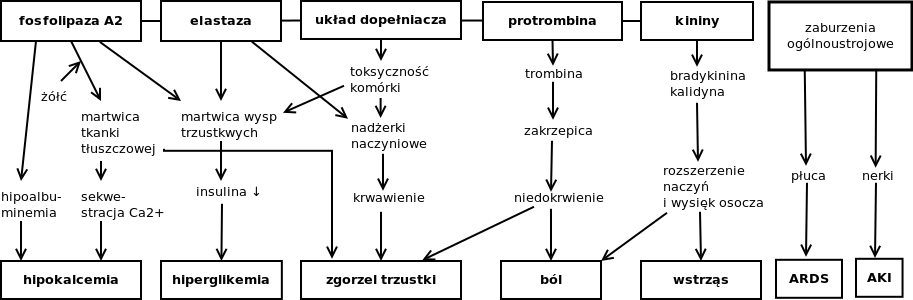
\includegraphics[scale=0.4]{pat_pan}
\caption{Patogeneza ostrego zapalenia trzustki}
\end{figure}

Niszczone są również sąsiadujące tkanki. Rozwija się martwica tkanki
tłuszczowej z towarzyszącym powstawaniem mydła, w wyniku czego
zużywane są jony Ca$^{2+}$, co może być przyczyną
hipokalcemii. Uwolnione kwasy tłuszczowe wiążą się z kolei z jonami
Mg$^{2+}$, powodując hipomagnezemię. Martwica może rozszerzać się
również na inne okoliczne narządy. Może dojść do niedrożności i/lub
perforacji przewodu pokarmowego, zapalenia otrzewnowej. Objęcie
procesem zapalnym okrężnicy może być przyczyną translokacji
bakteryjnej i wtórnej infekcji.

Wyciek enzymów do krwi prowadzi do hipoalbuminemii z następczą
hipokalcemią, a także do uogólnionego rozszerzania naczyń i tworzenia
wysięków (bradykinina, kalidyna), co może prowadzić do
wstrząsu. Fosfolipaza A$_2$ i wolne kwasy tłuszczowe (powstające w
wyniku nasilonej lipolizy) niszczą surfaktant nabłonka pęcherzyków
płucnych prowadząc w efekcie do hipoksji.

Przyczyny wstrząsu w ostrym zapaleniu trzustki są
wielorakie. Początkowo dochodzi, w wyniku miejscowego zapalenia do
przemieszczania się płynu w postaci przesięku do
przestrzeni zaotrzewnowej i/lub jamy otrzewnowej. Wynikiem
niedrożności jelit jest sekwestracja płynu w przewodzie
pokarmowym. Deficyt płynowy nasilają wymioty i trudności w przyjmowaniu
płynów drogą doustną. Uogólniony proces zapalny (SIRS) powoduje
rozszerzenie łożyska naczyniowego i wzrost przepuszczalności naczyń.
Hipokalcemia może być przyczyną niewydolności sercowo-naczyniowej.

\chapter{Objawy i rozpoznanie}

Najbardziej typowym objawem ostrego zapalenia trzustki jest ból
brzucha - bardzo silny, zlokalizowany w nadbrzuszu, często
promieniujący do kręgosłupa (jest to związane z zaotrzewnowym
położeniem trzustki). Bólowi prawie zawsze towarzyszą nudności i
nieprzynoszące ulgi wymioty. Dość częstym objawem jest gorączka, która
w pierwszym tygodniu jest wynikiem SIRS, a w późniejszym okresie może
być objawem infekcji. W przypadku chorób dróg żółciowych obecna może
być żółtaczka. W badaniu fizykalnym można stwierdzić objawy
otrzewnowe, brak perystaltyki, hipotensję, ściszenie szmerów oddechowych nad płucem
(częściej lewym), związane z wysiękiem w jamie opłucnowej, zaburzenia
świadomości, będące wynikiem wstrząsu, hipoksemii i endotoksemii 
oraz różnorodne objawy skórne: zaczerwienienie twarzy (objaw
Loeflera), sinica twarzy i kończyn, zasinienia w okolicy pępka (objaw
Cullena) lub w okolicy lędźwiowej (objaw Greya-Turnera).

Ostre zapalenie trzustki rozpoznaje się dzięki obecności powyższych
objawów i wzrostu osoczowych poziomów enzymów trzustkowych, czyli amylazy i
lipazy. Wysokie stężenie lipazy jest bardziej czułym i swoistym
markerem ozt. Poziomy obydwu enzymów zazwyczaj wracają do normy po 2-3
dniach od początku objawów, pomimo trwania choroby. Przez dłuższy czas
natomiast utrzymuje się zwiększona aktywność amylazy całkowitej w moczu oraz
aktywność izoformy trzustkowej tego enzymu we krwi. W USG jamy
brzusznej trzustka, jeśli uda się ja uwidocznić, może być powiększona,
jej granice zatarte, a miąższ może być niejednorodny echogenicznie.

Złotym standardem w rozpoznawaniu ostrego zapalenia trzustki jest
tomografia komputerowa z podaniem środka kontrastującego. Badanie to
pozwala również ocenić stopień ciężkości choroby (tabela nr 2) i
wykryć niektóre powikłania. Na podstawie obrazu TK można wyliczyć
tzw. tomograficzny wskaźnik ciężkości ostrego zapalenia
trzustki (\textsl{CTSI - CT severity index}). Martwicę trzustki na ogół można
uwidocznić w TK dopiero po 72 godzinach od początku choroby, dlatego
wcześniejsze badanie może nie dostarczyć wiarygodnych informacji co do
stopnia nasilenia zmian martwiczych. Najlepiej wykonać to
badanie dopiero po 5-7 dniach od początku choroby, szczególnie w
przypadku gdy istnieją wątpliwości diagnostyczne, objawy kliniczne są
bardzo nasilone, w razie braku poprawy po 72 godzinach
konwencjonalnego leczenia, w przypadku gdy dochodzi do gwałtownego pogorszenia stanu
pacjenta po wstępnej poprawie oraz przy punktacji powyżej 3 punktów w
skali Ransona lub powyżej 7 w skali APACHE II.

\begin{table}[htbp]
\begin{center}
\begin{footnotesize}
\begin{tabular}{|c p{9cm} c|}
\hline
\multicolumn{3}{|c|}{\cellcolor[gray]{0.9} \textbf{Tabela 2. Stopnie TK i tomograficzny
  wskaźnik ciężkości OZT$^\star$ (CTSI)}}\\
\hline \hline
Stopień & Objawy & Punkty\\
\hline \hline
A & prawidłowy obraz trzustki & 0\\
\hline
B & zmiany zapalne ograniczone do trzustki & 1\\
\hline
C & zmiany zapalne w obrębie trzustki i sąsiadujących tkanek & 2\\
\hline
D & bardziej zaawansowane zmiany zapalne obejmujące trzustkę,
    okoliczne tkanki oraz 1 niewyraźnie odgraniczony zbiornik płynowy
    okołotrzustkowy & 3\\
\hline
E & mnogie lub rozległe zbiorniki płynu zlokalizowane poza trzustką
    lub zainfekowany zbiornik płynu & 4\\
\hline \hline
Martwica (\%) & & Punkty\\
\hline \hline
0 & & 0\\
< 33 & & 2\\
33 - 50 & & 4\\
$\geq$ 50 & & 6\\
\hline \hline
\multicolumn {3}{|p{13cm}|}{\textbf{CTSI (0 - 10 pkt)} - punktacja TK + punktacja
  martwicy; wynik $\geq$7pkt wskazuje na ciężki przebieg i duże ryzyko
  zgonu}\\
\hline
\multicolumn {3}{|p{13cm}|}{\scriptsize{$^\star$ stopnie TK określa się
  na podstawie niewzmocnionego obrazu TK, stopień zaawansowania martwicy po podaniu
  kontrastu}}\\
\hline
\end{tabular}
\end{footnotesize}
\end{center}
\end{table}

Wczesna identyfikacja pacjentów z ryzykiem wystąpienia ciężkiego
zapalenia trzustki pozwala na dokładne monitorowanie przebiegu
choroby, pomaga także w ustaleniu rokowania. Istnieje wiele narzędzi
służących do określania ryzyka u pacjentów z ozt. Należą do nich skala
Ransona (tabela nr 3) i Glasgow (tabela nr 4). Pomimo stosunkowo dużej
popularności wartość kliniczna, szczególnie w zakresie rokowania jest
niewielka.

\begin{table}[!h]
\begin{center}
\begin{footnotesize}
\begin{tabular}{|l l l|}
\hline
\multicolumn{3}{|c|}{\cellcolor[gray]{0.9} \textbf{Tabela 3. Kryteria Ransona}}\\
\hline \hline
\multicolumn{2}{|l}{\textbf{Przy przyjęciu do szpitala}} & \\
\hline
 & \multicolumn{2}{l|}{Wiek >55 lat}\\
 & \multicolumn{2}{l|}{Leukocytoza >16000/mm$^3$}\\
 & \multicolumn{2}{l|}{Glikemia >200 mg/dl (10 mmol/l)}\\
 & \multicolumn{2}{l|}{LDH >350 j./l}\\
 & \multicolumn{2}{l|}{AspAT >250 j./l}\\
\hline \hline
\multicolumn{2}{|l}{\textbf{W ciągu pierwszych 48 godzin}} & \\
\hline
 & \multicolumn{2}{l|}{Spadek hematokrytu o ponad 10\%}\\
 & \multicolumn{2}{l|}{Wzrost poziomu mocznika o ponad 5 mg/dl }\\
 & \multicolumn{2}{l|}{Stężenie wapnia <8 mg/dl (2 mmol/l)}\\
 & \multicolumn{2}{l|}{PaO$_2$ <60 mmHg (8 kPa)}\\
 & \multicolumn{2}{l|}{Niedobór zasad >4 mEq/l}\\
 & \multicolumn{2}{l|}{Sekwestracja płynów >6 l}\\
\hline \hline
\parbox[b]{3cm}{\textbf{Liczba\\objawów}} & \parbox[b]{3cm}{\textbf{Odsetek\\powikłań}}
 & \parbox[b]{3cm}{\textbf{Śmiertel-\\ność}}\\
\hline
<2 & <5\% & <1\%\\
3-5 & 30\% & 5\%\\
>6 & 90\% & 20\%\\
\hline
\end{tabular}
\end{footnotesize}
\end{center}
\end{table}

\begin{table}[!h]
\begin{center}
\begin{footnotesize}
\begin{tabular}{|l l|}
\hline
\multicolumn{2}{|c|}{\cellcolor[gray]{0.9} \textbf{Tabela 4. Skala Glasgow}}\\
\hline \hline
\multicolumn{2}{|l|}{\textbf{W ciągu pierwszych 48 godzin}}\\
\hline
 & Wiek >55 lat\\
 & Leukocytoza >15000/mm$^3$\\
 & AspAT >200 j./l\\
 & LDH >600 j./l\\
 & Glikemia >180 mg/dl (10 mmol/l)\\
 & Albuminy <32 g/l\\
 & Stężenie wapnia <8 mg/dl (2 mmol/l)\\
 & PaO$_2$ <60 mmHg (8 kPa)\\
 & Stężenie mocznika >45 mg/dl (16 mmol/l)\\
\hline \hline
\multicolumn{2}{|p{10cm}|}{\textsl{Obecność 3 lub więcej objawów wskazuje na ciężkie
  zapalenie trzustki}}\\
\hline
\end{tabular}
\end{footnotesize}
\end{center}
\end{table}

Skala POP (\textsl{Pancreatitis Outcome Prediction Score}) jest
przydatnym, w szczególności w połączeniu z oceną tomograficzną
narzędziem rokowniczym. Oceniane jest 6
parametrów (tj. wiek, MAP, PaO$_2$/FiO$_2$, pH krwi, poziom mocznika i
wapńa w osoczu), oznaczanych w pierwszych 24 godzinach od początku
choroby. W zależności od ilości punktów można określić ryzyko zgonu.

Obecnie najprzydatniejszą skalą stosowaną w ocenie ciężkości przebiegu
ozt jest skala Marshalla (tabela nr 6), opierająca się na założeniu,
że najpewniejszym wskaźnikiem ciężkości ostrego zapalenia trzustki
jest niewydolność narządowa, która utrzymuje się ponad 48 godzin.
Oceniane są trzy najczęściej występujące uszkodzenia narządowe,
występujące w przebiegu OZT, czyli niewydolność krążenia, oddechowa i
nerek.

\begin{table}[!h]
\begin{center}
\begin{footnotesize}
\begin{tabular}{|p{3cm} | p{0.8cm} p{2.4cm} p{2.6cm} p{1.4cm} p{1.3cm}|}
\hline
\multicolumn{6}{|c|}{\cellcolor[gray]{0.9} \textbf{Tabela
  5. Zmodyfikowana skala Marshalla}}\\
\hline \hline
 & \multicolumn{5}{l|}{\textbf{Punktacja}}\\
\cline{2-6}
\textbf{Układ} & 0 & 1 & 2 & 3 & 4\\
\hline
oddechowy & \multicolumn{5}{l|}{}\\
 (PaO$_2$/FiO$_2$) & >400 & 301-400 & 201-300 & 101-200 & $\leq$100\\
\hline
nerki (kreatynina w surowicy)$^\star$ & \multicolumn{5}{l|}{}\\
<$\mu$mol/l> & $\leq$134 & 134-169 & 170-310 & 311-439 & > 439\\
<mg/dl> & $\leq$1,4 & 1,4-1,9 & 1,92-3,5 & 3,51-4,96 & >4,96\\
\hline
krążenia (skurczowe ciśnienie tętnicze, mmHg)$^\star$$^\star$ 
& >90 & <90 odpowiedź na resuscytację płynową 
& <90 brak odpowiedzi na resuscytację płynową 
& < 90,\newline pH <7,3 & <90,\newline pH <7,2\\ 
\hline \hline
\multicolumn{6}{|p{13cm}|}{\textsl{Wynik $\geq$2 dla któregokolwiek układu
  oznacza ,,niewydolność narządową''}}\\
\hline
\multicolumn{6}{|p{13cm}|}{\scriptsize{$^\star$punktacja u chorych z istniejącą przewlekłą
  niewydolnością nerek zależy od stopnia pogorszenia wyjściowej
  czynności nerek\newline $^\star$$^\star$bez wspomagania inotropowego}}\\
\hline
\end{tabular}
\end{footnotesize}
\end{center}
\end{table}

Oczywiście stosowane są również bardziej uniwersalne skale oceny
ryzyka i ciężkości stanu pacjenta, w szczególności skala APACHE II
(wynik powyżej 8 punktów oznacza ciężkie zapalenie trzustki).

Wszystkie wymienione wyżej narzędzia są używane celem identyfikacji
pacjentów z ciężkim OZT, którzy powinni być od początku bardzo
intensywnie leczeni i monitorowani. Gdy niewydolność narządowa
występuje w przeciągu pierwszych 24 godzin i nie jest wiadome, czy
będzie ona przejściowa, czy przetrwała, należy pacjenta traktować jak
chorego na ciężką postać zapalenia trzustki. Zalecane jest powtórzenie
oceny ciężkości OZT po 24 i 48 godzinach oraz 7 dniach od przyjęcia do
szpitala.

\chapter{Leczenie}

\begin{thebibliography}{99}
\bibitem{7} Numer 7 z Parillo
\bibitem{szczeklik} Szczeklik \& co
\bibitem{traczyk} Traczyk
\bibitem{bochenek} Bochenek w/g wikipedii
\bibitem{banks} Banks P.A., Bollen T.L., Dervenis C., et al.; Acute
  Pancreatitis Classification Working Group. Classification of acute
  pancreatitis – 2012: revision of the Atlanta classification and
  definitions by international consensus. Gut, 2012; 62: 102–111
\bibitem{38} Parillo 38
\bibitem{39} Parillo 39
\bibitem{40} Parillo 40
\bibitem{21} Parillo 21
\bibitem{27} Parillo 27
\bibitem{26} Parillo 26
\end{thebibliography}
\addcontentsline{toc}{chapter}{Bibliografia}
\end{document}